\newlength{\bibsep}
\documentclass[nonatbib,5p,a4paper]{elsarticle}  % 5p for two columns, 1p for 1 column (this is specific for the elsearticle)
\usepackage[english,norsk,nynorsk]{babel}        % Language
\usepackage[DatePublished]{Code/NTNU-lab}        % remove [DatePublished] to remove dates
\usepackage{csquotes}                            % Must be loaded when babel is loaded to avoid error.
% Use this file to write code that you do not want in the .sty file, but has to be in the preamble (before \begin{document}).
% Writing in this file in stead of in the preamble will keep the main file more organised and tidy.


%                       Nomenclatures
%_______________________________________________________________
\usepackage[intoc]{nomencl}
\makenomenclature
\usepackage{listings}
\renewcommand{\nomname}{%
% Title
%----------------
List of Symbols
%----------------
}
\renewcommand{\nompreamble}{%
% Description
%----------------
The next list describes several symbols that will be later used within the body of the document
%----------------
}
% This code creates the groups
\renewcommand\nomgroup[1]{%
  \item[\bfseries
  \ifstrequal{#1}{A}{Physics constants}{%
  \ifstrequal{#1}{B}{Mathematical constants}{%
  \ifstrequal{#1}{C}{Other symbols}{}}}%
]}
% This will add the units
\newcommand{\nomunit}[1]{%
\renewcommand{\nomentryend}{\\#1}}
%................................................................

                            % Write all preamble code in this file to keep it organised and tidy.

\addbibresource{Bibliography/Sources.bib}        % Selects the Bibliography file.


\begin{document}
\selectlanguage{english}                         % Sets the language of the document.

%%%%%%%%%%%%%%%%%%%%%%%%%%%%%%%%%%%%%%%%

\begin{frontmatter}
%
% Title:
%------------------------------------
\title{%
Final Report\\
\small For individual project  % A good idea is to have the subject code and name as subtitle
}
%
% Authors:
%------------------------------------
% List an author with name ' Firstname Middlename Lastname ' like this:
% F. M. Lastname
\author{Jonas Brami} 
\author{Brett Stevens}

%
% Date:
%------------------------------------
%
\newdate{dateName}{31}{08}{2022} % edit the date here, ' dateName ' has to match on these two lines.
\renewcommand*{\today}{\DayMonthYearDateFormat\displaydate{dateName}} 
% Options for displaying date: \MonthYearDateFormat,  \DayMonthYearDateFormat or \YearDateFormat
%
% Abstract:
%------------------------------------
%
\end{frontmatter}
%
%
% Table of contents:
%------------------------------------
% If the report is very long for some reason (over 4 or 5 pages), use a table of contents.
% Uncomment everything below the line ---- to get table of contents (ctrl + /) (the / on numberpad):
%-------------

\ 
\vspace{1cm}

\begin{minipage}{\textwidth}
    \tableofcontents
\end{minipage}
\clearpage
\section{Introduction}
% Delete the text and write your Introduction here:
%------------------------------------




The problem we aim to solve during this project is the placement of a sensor on a specific target point on a surface using a fixed manipulator arm mounted on the top of an unmanned quadcopter.
A quacopter is an underactuacted helicopter with four rotors. This UAV (Unmanned Aerial Vehicles) is underactuated because arbitrary configurations and trajectory cannot be realized.\\
In the last ten years, research about UAV controls accelerated drastically with many applications in the civilian industry in a variety of areas.\\
Monitoring and sensing tasks are traditionally operated by human but they be complicated, expensive and dangerous for the human operator when the point of interest is hard to reach. For example, big structures like bridges need to undergo regular inspections to ensure there are no cracks or other signs of structural fatigue.\\
Using UAVs for such tasks would not only reduce cost of maintance of those structures, but also increase the security of both the human manipulator and the civilians using it. \\
Sensor placement on surfaces using UAVs  is an active field of research and we will propose a solution based on velocity fields.\\

A velocity field is a function taking as input  a four dimensional vector $(x,y,z,t)$ and returning a 3 dimensional velocity vector $(u,v,w)$.\\
Since our environment is static, meaning that the obstacles and goal are not moving, we will always use a time invariant velocity field.
Diverse ways of placing sensors using UAVs have been explored in the past, including but not limited to: 
\begin{itemize}
    \item Direct Placement: Using a fixed arm manipulator on an UAV, we use the force exerted by the thrust of the UAV to provide enough pressure on the tip of the arm to place the sensor on the target point.
    \item Sensor Launching \cite{farinha2020unmanned}: Using the energy stored in a spring, the UAV ejects the sensor at the desired velocity to reach and attach to the target (Unmanned Aerial Sensor Placement for Cluttered Environments). This strategy is very useful when it is not physically possible for a mounted arm to reach the target however it suffers from small payload capacity.
    \item Drop from flight: We simply drop the sensor above the target point. When target accuracy is not a priority and we are aiming at a non-vertical surface and there is no occlusion above the target,  this sensor placement strategy is the most effective. 
\end{itemize}
\begin{figure}[h!]
    \centering
    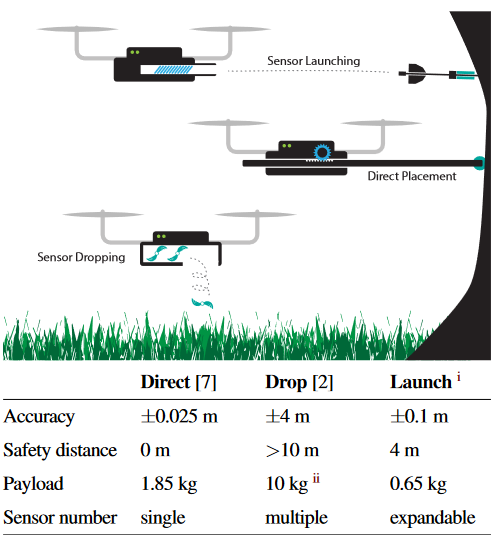
\includegraphics[width=0.48\textwidth]{Images/threeway.png}
    \caption{Different types of sensor placement from \cite{farinha2020unmanned}}
    \label{fig:threeway}
\end{figure}
The characteristics of each one of mentioned methods are shown in \ref{fig:threeway}.
We decided to go through with the Direct Placement strategy because despite its simplicity, it provides good accuracy and is able to place a large variety of payloads. 
The solution we will propose can be divided in 3 parts: The first is environment mapping where we perform surface and obstacle recognition using live depth sensor feed. The second part is designing a potential based velocity field to perform path-planning by guiding the UAV from the start point to the target point. The third and last part is designing a velocity field around the target point to apply the desired force amplitude. In this part, we will use the passive velocity field controller (PVFC) to optimize our energy consumption.

\section{Background and Literature Review}
% Delete the text and write your Theory/ Background Information here:
%------------------------------------
\subsection{Placing sensors using UAVs}
Diverse ways of placing sensors using UAVs have been explored in the past, including but not limited to: 
\begin{itemize}
    \item Direct Placement: Using a fixed arm manipulator on an UAV, we use the thrust of the UAV to provide enough pressure on the tip of the arm to place the sensor on the target point.
    \item Sensor Launching \cite{farinha2020unmanned}: Using the energy stored in a spring, the UAV ejects the sensor at the desired velocity to reach and attach to the target (Unmanned Aerial Sensor Placement for Cluttered Environments). This strategy is very useful when it is not physically possible for a mounted arm to reach the target, however, it suffers from small payload capacity.
    \item Drop from flight: We simply drop the sensor above the target point. When target accuracy is not a priority and we are aiming at a non-vertical surface and there is no occlusion above the target,  this sensor placement strategy is the most effective. 
\end{itemize}
\begin{figure}[h!]
    \centering
    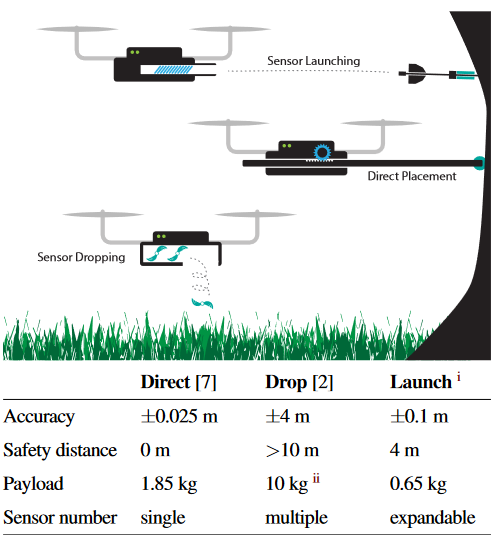
\includegraphics[width=0.48\textwidth]{Images/threeway.png}
    \caption{Different types of sensor placement from \cite{farinha2020unmanned}}
    \label{fig:threeway}
\end{figure}

The characteristics of each one of mentioned methods are shown in figure \ref{fig:threeway}.
We decided to go through with the Direct Placement strategy because despite its simplicity, it provides good accuracy and is able to place a large variety of payloads.\\

\subsection{Current State of the art for UAM}
There exists 2 main approaches for controls of unmanned aerial manipulators: The first one is the centralized approach where we consider the manipulator and the UAV as a whole; whereas in the decentralized approach, the manipulator controls and UAV control are independant problems.
In the case of the Sensor placement with a quadcopter, we use the centralized approach because the arm has no degree of freedom and the force exerted by the tip is coming from the thrust of the UAV.
The centralized approach is often built on top of a model-based full state control loop optimized with LQR (Linear–quadratic regulator) around some desired state. 
In \cite{ruggiero2018aerial}, the author present the current state of the research for UAMs.
An UAM can be divided into 4 elements: the UAV floating base (in our case, a quadcopter), the robotic arm, a sensor/gripper attached to the end of the arm (in our case, a sensor will be attached to the end of the arm), diverse sensors on UAV to handle perception (the depth camera).
While the state of the art approaches for UAV controllers are based on minimizing a state trajectory error, the planning strategy we will study next is based on velocity fields.
\subsection{Velocity field path-planning for single and multiple unmanned aerial vehicles}
In \cite{farinha2020unmanned}, the author presents a path-planning technique based on velocity fields generated from potentials solution of Laplace's equation.
Two different types of solution to potential $V$ for the Laplace 
\begin{align} % Use & sign to align, use \nonumber to write a line without number.
    \laplacian{V} &=0 \nonumber \\
    \frac{\partial^2 V}{\partial x^2}+\dpd[2]{V}{y} &=0 \label{eq:Laplace} % dpd = display mode partial derivative
\end{align}
equation are presented in this paper: Type 1 are irrotational solutions to generate sink and source fields and Type 2 solutions are used to build solenoidal fields.
\begin{align} % Use & sign to align, use \nonumber to write a line without number.
    {V}_{1} = {Q}_{1} \ln(({x}_{1}-\tilde{{x}_{1}})^2+({x}_{2}-\tilde{{x}_{2}})^2) \\
    {V}_{2} = {Q}_{2} \arctan(\frac{({x}_{2}-\tilde{{x}_{2}})}{({x}_{1}-\tilde{{x}_{1}})})
\end{align}
where $({x}_{1},{x}_{2})$ is the position of the UAV, $(\tilde{{x}_{1}}, \tilde{{x}_{2}})$ is the position of the obstacle;
${V}_{1}$ and ${V}_{2}$ are respectively type 1 solution (source field) and type 2 solution (vortex field). \\
The author justifies the use of Laplace solution for building the velocity field for multiple reasons:
\begin{itemize}
    \item The use of Laplace solution for potential guarantees the uniqueness of the minimum in the field. 
    Specifically, the use of vortex function built from shaping function to circle around obstacle will
    ensure that only the goal point will be a minimum of the field and that the UAV will not get stuck at some local minimum. 
    As the author states, we can do an analogy to a famous strategy to find the exit of a maze: 
    by keeping a hand on a wall of the maze and walking while always touching the wall, we are ensured to find the end of the maze. 
    This is far from being an optimal solution, however, it can guarantee that the goal will be reached. 
    As a result, those solenoidal fields based on vortex function also provide active collision avoidance. 
    \item Scalar shaping functions are at the base of these methodology because by crafting them to match the shape of the obstacles, 
    we are able to generate corresponding vortex or repulsive functions for obstacles of any shape. 
    Since those functions are defined for each obstacle, it would be easy to reevaluate the field after addition or removal of an obstacle.
    \item Finally, irrotational solutions of the Laplace equation allow us to enforce an exclusion radius around obstacles (source field) and to direct the UAV in direction of the target point (sink field).
    The exclusion radius is encoded using the amplitude ${Q}_{1}$ of the irrotational field.
\end{itemize}

We can leverage these both types of potentials to derive a velocity field that will guide the UAV to the contact point without colliding with the surface.
For example, we could define the exclusion radius to be the distance between the centre of mass (CoM) of the quadcopter and its most distant part on the quadcopter. 

We will present the field we previously described with illustrations. 
\begin{figure}[h!]
    \centering
    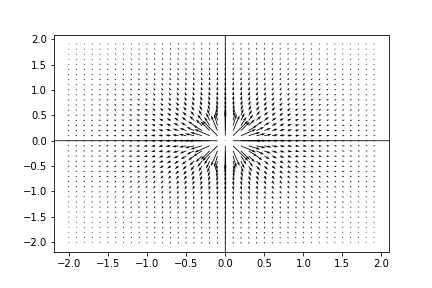
\includegraphics[width=0.48\textwidth]{Images/simplesource.png}
    \caption{Simple Type 1 irrotational source}
    \label{fig:simplesource}
\end{figure}
The field in figure \ref{fig:simplesource} was drawn by computing the gradient of $V_1$ with $(\tilde{{x}_{1}}, \tilde{{x}_{2}}) = (0,0)$.

\begin{figure}[h!]
    \centering
    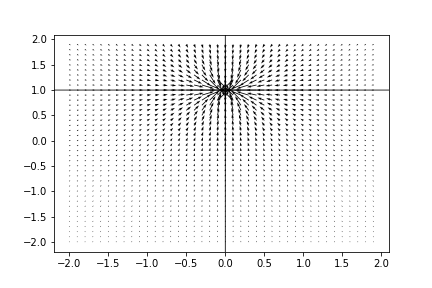
\includegraphics[width=0.48\textwidth]{Images/simplesink01.png}
    \caption{Simple Type 1 irrotational sink}
    \label{fig:simplesink}
\end{figure}
The field in figure \ref{fig:simplesink} is a sink field at $(0,1)$, it is similar to the source field in figure \ref{fig:simplesource} but with opposite sign.

\begin{figure}[h!]
    \centering
    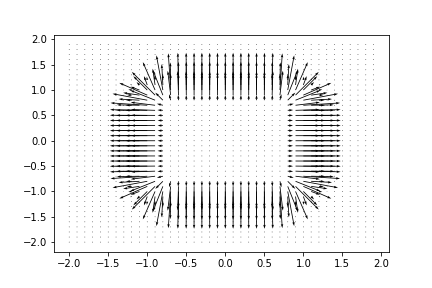
\includegraphics[width=0.48\textwidth]{Images/irrotafromshaping.png}
    \caption{irrotational field from shaping function}
    \label{fig:irrotafromshaping}
\end{figure}
The field in figure \ref{fig:irrotafromshaping} has been generated by computing the gradient of the shaping function of a superquadratic: 
\begin{align}
    H=(x_1-\tilde{{x}_{1}})^n+(x_2-\tilde{{x}_{2}})^n \\
    F=\frac{1}{1+(\frac{1}{L}H^{\frac{1}{n}})^m}
\end{align}
As stated in \cite{mcinnes2003velocity}, when $m\gg1$, the edge of the shaping function gets thinner. Higher values of $n$ result in more rectangular shapes whereas $n=2$ describes the shaping function of an infinite cylinder.

Both these fields are type 1 irrotational solutions of the Laplace equation.

By adding the irrotational sink from figure \ref{fig:simplesink} and the irrotational field from shaping function in figure \ref{fig:irrotafromshaping} we obtain a good representation in figure \ref{fig:irrotafromshapingwithsink} of what the velocity field will look like when close to the target point. 
\begin{figure}[h!]
    \centering
    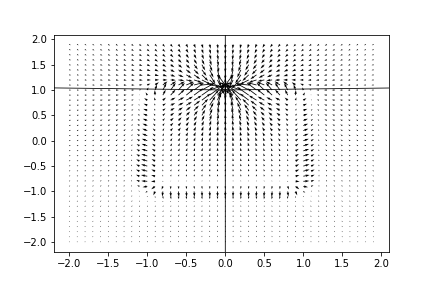
\includegraphics[width=0.48\textwidth]{Images/irrotashapingwithsink.png}
    \caption{irrotational field from shaping function with sink}
    \label{fig:irrotafromshapingwithsink}
\end{figure}

The shaping function is mainly used to generate a vortex field around an obstacle, as explained in the paper. It is given by: 
\begin{equation}
    v_2=-\frac{\partial{F}}{\partial{x_2}}e_1 + \frac{\partial{F}}{\partial{x_1}}e_2
\end{equation}
Here, $e_1$ and $e_2$ are an orthonormal basis. \\ 
We can see in figure \ref{fig:rotafromshaping} an example of vortex field around a super quadriatic.
\begin{figure}[h!]
    \centering
    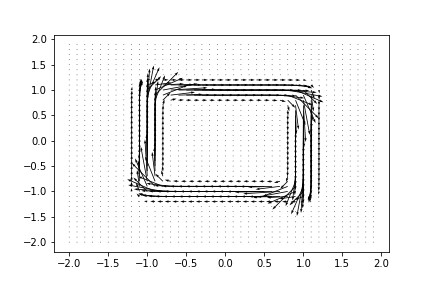
\includegraphics[width=0.48\textwidth]{Images/rotafromshaping.png}
    \caption{Solenoidale field from shaping function}
    \label{fig:rotafromshaping}
\end{figure}

\subsection{QUAD PD CONTROL example}


\section{Design and Theory}
\subsection{Designed velocity Field for planning task}
A velocity field is a function taking as input a state, $q$ and returns a 3-dimensional desired velocity vector $(u,v,w)$.\\ It describes a path (a function of position) as opposed to a trajectory (function of position and time).
\subsubsection{Sink field for reaching the target}
In \cite{mcinnes2003velocity}, the author chose to apply a logarithmic function on the distance between the current position and the goal position as a potential for the sink field. 
However, we observed that using such a potential does not allow the robot to safely approach the goal point since when the distance approaches 0, the logarithmic function diverges.
As a result, we decided to simply use the distance as a potential function. This will allow us to smoothly decrease the velocity of the UAV when approaching the desired goal point.
\subsubsection{Obstacle repulsive field}
In our current solution, because of the simplicity of the environement and the convexity of the obstacles, we are only using the type 1 solution described in \cite{mcinnes2003velocity}, we only have a repulsive field normal to the surface of the obstacle.
\subsubsection{Spherical field to maintain desired force }
When contact has been made, we suppose that the surface static friction coefficient is high enough to maintain the contact.
Since the arm has a fixed size and does not move, this section will describe a velocity field on the surface of a sphere around the target point with a radius defined by the distance between the CoM of the quadcopter and the tip of the arm.\\
First we need to compute the feasible position of the CoM to apply the desired force. 
We know that this position is unique because there is only one vertically stable pitch for a given desired force amplitude. The quadcopter needs to pitch to have a forward velocity because the quadcopter is underactuacted.\\
We can generate the velocity field on the surface of the sphere to point on the tangent direction of the sphere in the direction of the stable pitch position. \\
This field will have an amplitude proportional to the distance from this point.
The planning strategy we described would also allow us to easily define a desirable range for the yaw angle depending on the type of sensor and on the friction coefficient of the target surface.
Finally, we use a Passive Velocity Field Controller \cite{li1999passive} to follow this field to minimize the loss of kinetic energy to the environment when interacting with the surface.
Now we are going to describe how the spherical field is computed. 
Let us recall that the cartesian to spherical coordinate change of variable is defined as
\begin{equation} 
    r = \sqrt{x^2+y^2+z^2}\\ \nonumber 
\end{equation}
\begin{equation}
    \theta = \arccos(\frac{z}{r})\\\nonumber 
\end{equation}
\begin{equation}
    \label{transformation}
    \phi =
    \begin{cases}
        \arctan(\frac{y}{x}), & \text{if $x>0$},\\
        \arctan(\frac{y}{x}) + \pi, & \text{if $x<0$ and $y\geq 0$},\\
        \arctan(\frac{y}{x}) - \pi, & \text{if $x<0$ and $y<0$},\\
        \pi/2, & \text{if $x=0$ and $y>0$},\\
        -\pi/2, & \text{if $x=0$ and $y<0$},\\
        \text{not defined} , & \text{if $x=0$ and $y=0$}
    \end{cases}       
\end{equation}  
The jacobian defining the curvature of the sphere at each point for this transformation is 
\begin{align}
    J = \frac{\partial{(x,y,z)}}{\partial{(r,\phi,\theta)}} \nonumber\\
    J = \begin{bmatrix}
        \sin(\theta)\cos(\phi) & \cos(\theta)\cos(\phi) & -\sin(\phi)\\
        \sin(\theta)\sin(\phi) & \cos(\theta)\sin(\phi) & \cos(\phi)\\
        \cos(\theta) & -\sin(\theta) & 0\\
        \end{bmatrix}
        \label{jacobian}
\end{align}

Figure \ref{fig:spherical} represents an example of such a field where the red point is the optimal position to apply the pressure, the blue arrows are the velocity field vectors and the center of the sphere is the point where the force is applied

\begin{figure*}[h!]
    \centering
    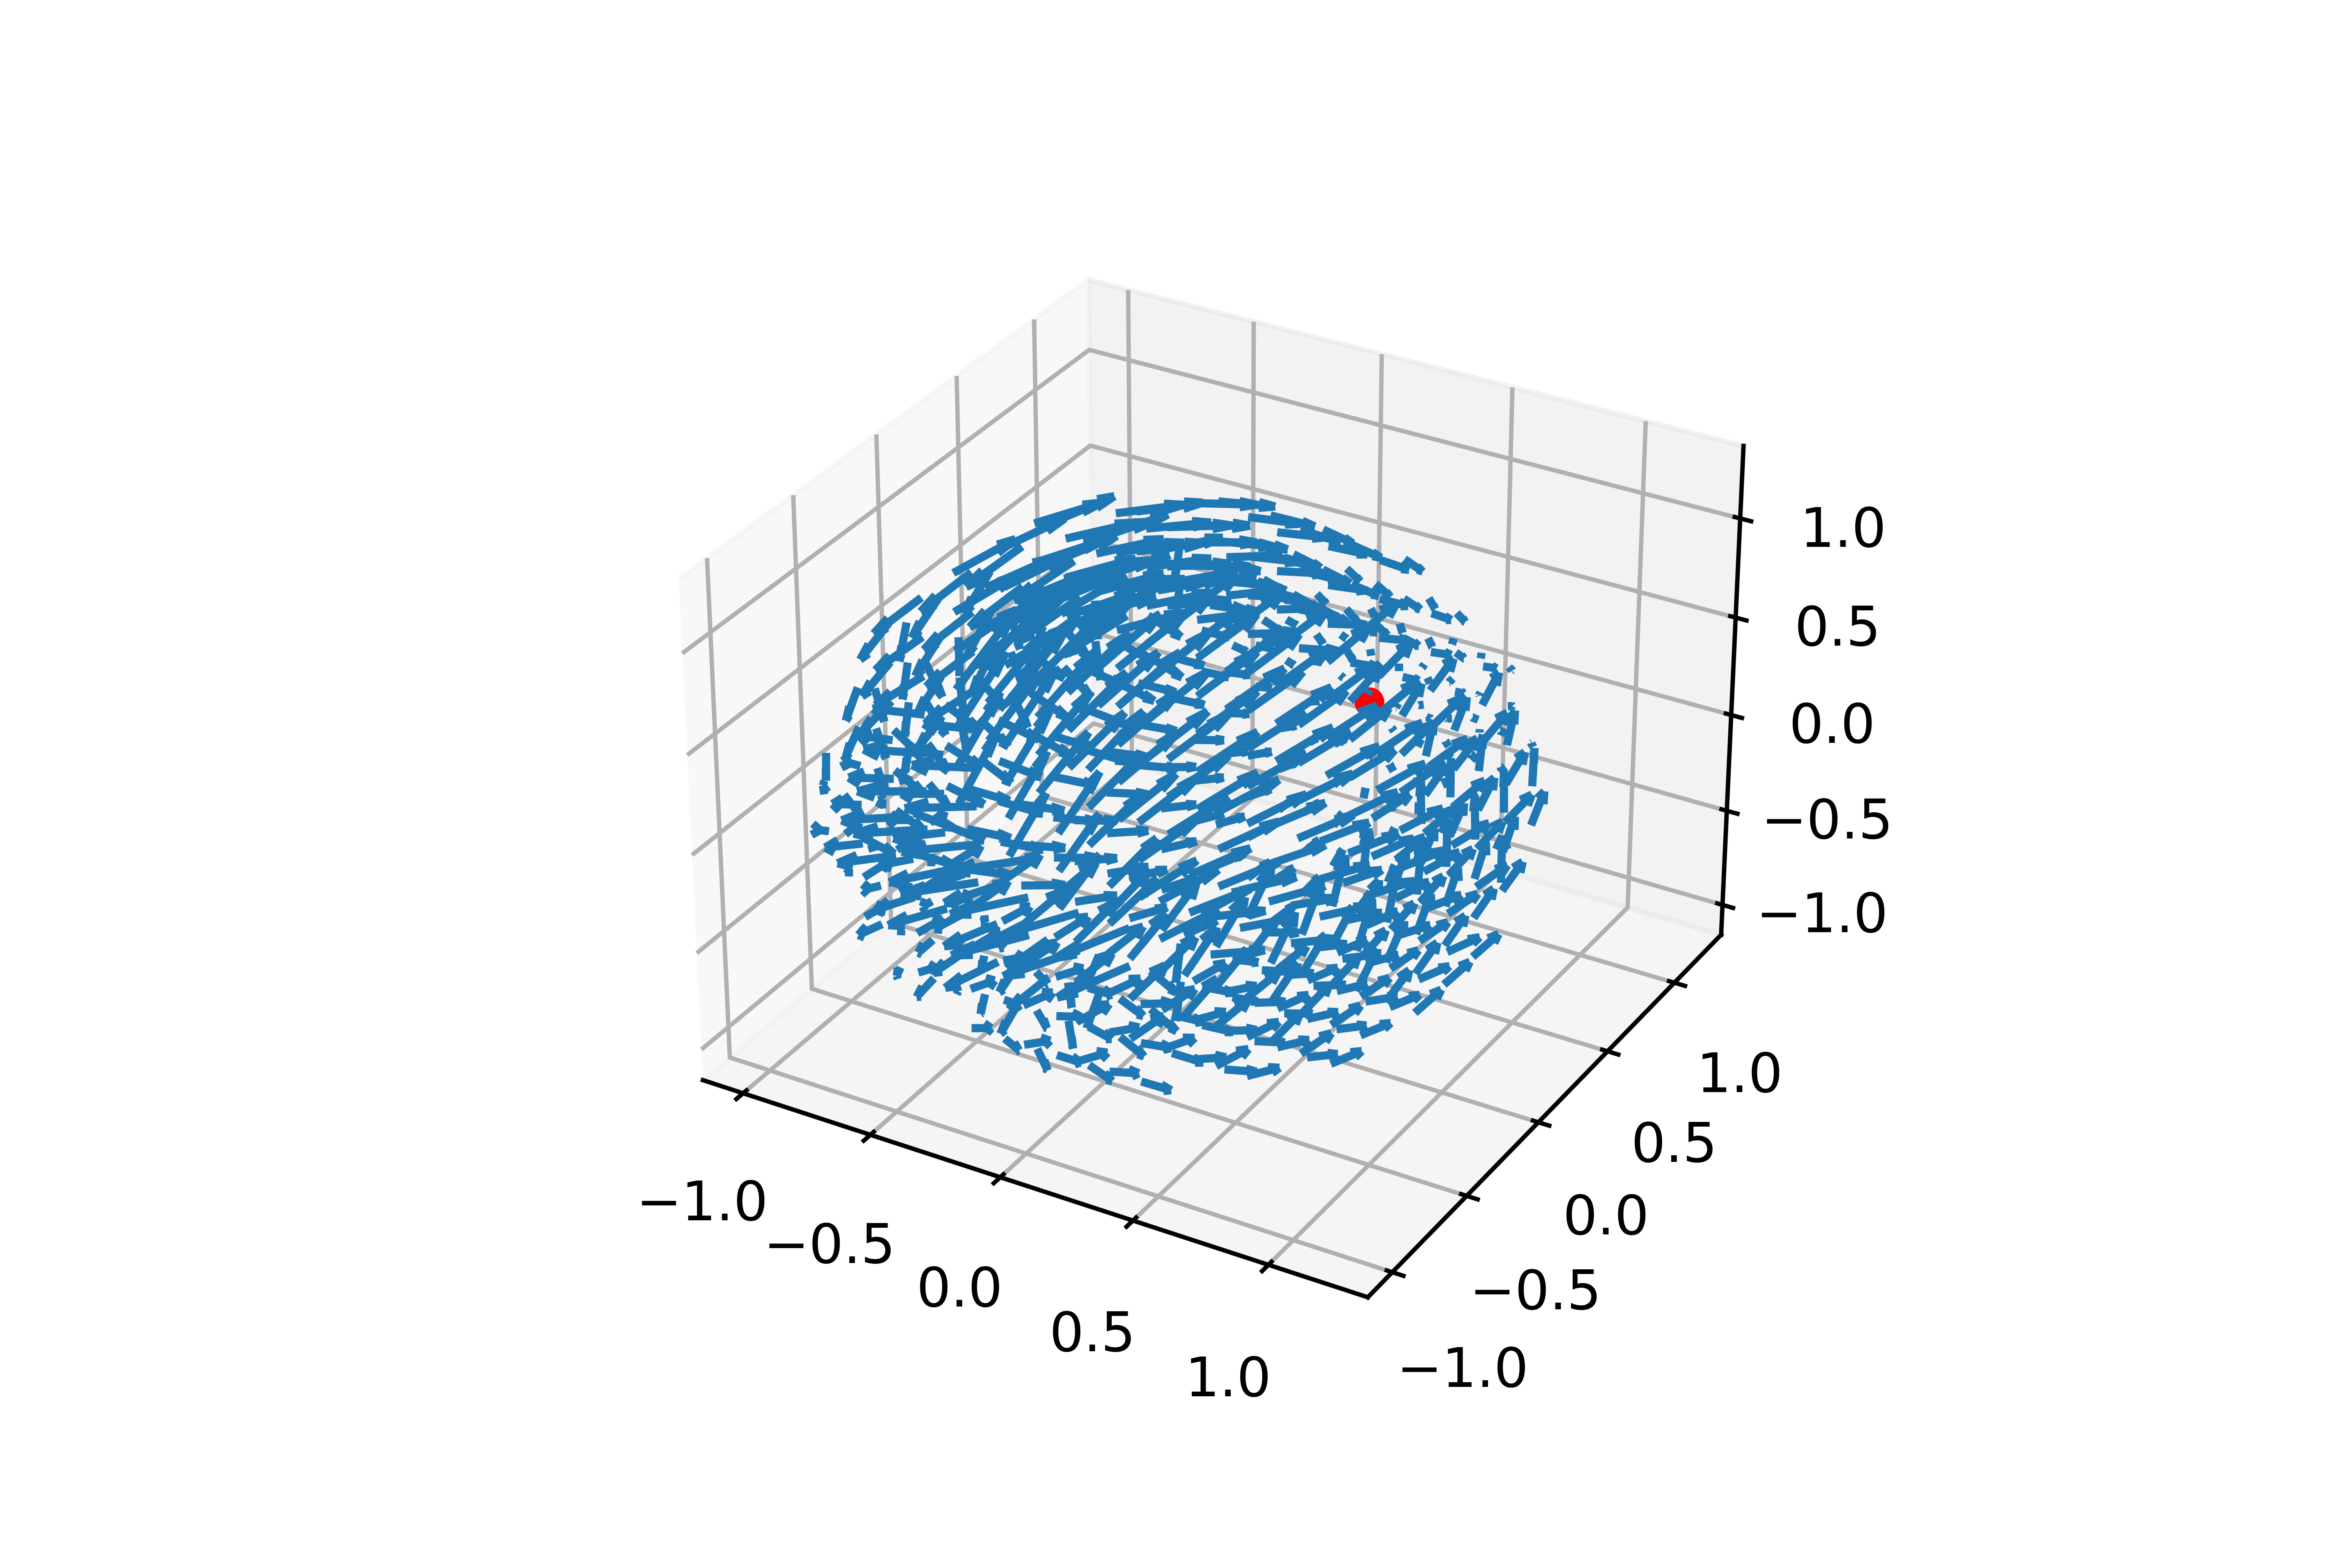
\includegraphics[width=\linewidth]{Images/sphericalfield.png}
    \caption{Spherical contact field}
    \label{fig:spherical}
\end{figure*}
\subsubsection{Circular field for contour following}
This field is based on the methodology explained in \cite{asl2019assistive}. We used it to build intuition, debug and analyze the controller.
The author explains how to encode a contour $\mathcal{C}$ into a desired velocity field $v_d$.
The field is given by: 
\begin{equation}
    v_d(p) = l(\alpha \hat{t} + \lVert Q-p \rVert \hat{n}) \label{eqn:circularfieldcons}
\end{equation}
\begin{itemize}
    \item $p\in \mathbb{R}_3$ is the current position
    \item $Q$ is the closest point from $p$ on $\mathcal{C}$
    \item $l , \alpha \in \mathbb{R}_{\geq 0}$ are scaling constants
    \item $\hat{t}$ is a unitary tangent vector to $\mathcal{C}$ at $Q$
    \item $\hat{n}$ is a unitary normal vector to $\mathcal{C}$ going from $p$ to $Q$
\end{itemize}

\begin{figure}[h!]
    \centering
    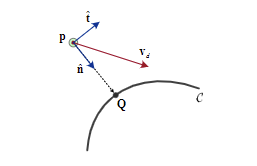
\includegraphics[width=0.48\textwidth]{Images/fieldconstruction.png}
    \caption{field construction from \cite{asl2019assistive}}
    \label{fig:fieldconstruction}
\end{figure} 

From there it is straightforward how to implement a circular velocity field with a radius of 1 and centered at the origin in the following way:
\begin{align}
    Q = \frac{p}{\sqrt{p_x^2 + p_y^2}}\\
    \theta = \arctan(Q_y, Q_x) \\
    \hat{t} = (-\sin{\theta}, \cos{\theta}, 0) \\
    \hat{n} = \frac{Q-p}{\lVert Q-p \rVert}
\end{align}
\subsection{Quadcopter modeling}
\subsubsection{Platform}
Similarly to the platform used in "An Aerial Parallel Manipulator with Shared Compliance", our system is composed of two subsytems: The underactuated quadrotor base (for which we have software in the loop integration given by PX4) and the fixed manipulator arm above the center of mass of the quad.
This system is underactued because in the base frame of this quad, the only thrust direction for the quadcopter is in the $z$ axis in the frame of the base of the quad, the rotors cannot move relative to the base of the quad. Therefore, the IRIS model control inputs are a quarternion vector and a thrust amplitude. However, the output of the passive controller for the non-augmented translational domain is a thrust vector $\Lambda \in\mathbb R_3 $, therefore we will need to convert this desired thrust to the desired format.
In addition to the fixed manipulator arm, a depth camera is mounted on the quad base. We use the depth camera model provided by Pixhawk 4 with IRIS that simulates an intel realsense r200. We use the transform provided in the PX4 obstacle avoidance package to transform from the frame of the camera to the frame of the quadcopter base, and we use the PX4 odometry information to transform from the base to the ground gazebo frame.

\subsubsection{Translational dynamics}

The dynamics that we take into account in our passive control strategy are only in the translational domain. The passive velocity field controller output is a thurst vector and PX4 translates this desired thurst into actual angular velocities for each one of the rotors 
$\Omega = (\bar{\omega_1}, \bar{\omega_2}, \bar{\omega_3}, \bar{\omega_4})$. PVFC only acts on the translational level and not at the rotational level and has no knowledge or control about the speed of thoses rotors and therefore the passivity of this controller is only at the translational level. 
This quadcopter is an underactuacted system because for a given translational velocity, only a subset of attitudes are feasible. As a result, it is not possible to control all 6 degrees of freedom independantly (3 translational, 3 rotational).
 
\subsection{Passive Velocity Field Control of Mechanical Manipulators}
In \cite{li1999passive}, the author explains the advantages of encoding a contour following task using velocity fields. 
They later present the passive velocity field controller whose objective is to "maintain an energetically passive relationship between the manipulator under closed loop control and
its physical environment, while causing the manipulator to perform the desired task." 
We will explain each one of those arguments and relate them to our sensor placement task.
\subsubsection{Velocity fields for planning}
The classical approach to do planning is to encode the task into a timed trajectory $Q:\mathbb R_{\ge 0} \rightarrow G$ where G is the n-dimensional configuration manifold for the manipulator and uses a controller to minimize the state trajectory error.
Using this strategy, the objective of the controller is to minimize the deviation between $q(t)$ and $Q(t)$ where $q:\mathbb R_{\ge 0} \rightarrow G$ is the actual coordinate representation of the manipulator.
This strategy could be fine if the manipulator was able to never deviate from the timed trajectory defined by Q. However, if deviation occurs for example, when external forces are applied to the
robot, a side effect of this minimization strategy called radial reduction can occur.

\begin{figure}[h!]
    \centering
    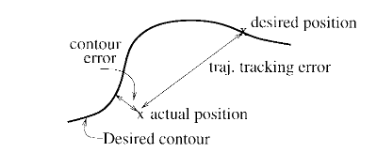
\includegraphics[width=0.48\textwidth]{Images/radialreduction.png}
    \caption{radial reduction from \cite{li1999passive}}
    \label{fig:radialreduction}
\end{figure} 
The author argues that if following the path of the desired trajectory is more important than the timing in which the manipulator follows this trajectory, a strategy based on velocity field is more appropriate because the velocity of the manipulator will only depend on its current position and will be time invariant.  
For the sensor placement task, using a timed trajectory strategy with deviation minimization to reach the contact point may lead the UAV to collide with an obstacle. With our strategy based on potential velocity field, the UAV will not try to shortcut the desired path in case of deviation.
The author defines an $\alpha$ error such that:
\begin{equation}
    e_{\alpha} = \dot{q} - \alpha V \label{alphaerror}
\end{equation}
One of the most important priorities of PVFC is that when no external forces are applied on the robot, there is a positive $\alpha$ such that 
\begin{equation}
    \lim_{t\to\infty}e_{\alpha} = 0
\end{equation}
In other words, PVFC does not seek to exactly match the desired velocity field but just an $\alpha$ scaled version of it. The $\alpha$ we are going to converge to is a function of the energy in the augmented system and the energy in the desired velocity field.
\subsubsection{Passivity}
The controller presented in this paper is based on energy control theory and allows energy transfer between the environement and the augmented system.
Passivity allows dissipation from the energy input to the system into the augmented system. \\
To present this concept, the author first defines the notion of a passive dynamic system:\\
A dynamic system with input $u \in U$ and output $y \in Y$ is passive with respect to the supply rate 
$s:U \cross Y \rightarrow \mathbb R$, if for any $u: \mathbb R_{\ge 0} \rightarrow U $ and for any $t\geq 0$ the following relation is satisfied:
\begin{align}
    \exists ~ c\in\mathbb R  \nonumber\\
    \int_{0}^{t}s(u(\tau),y(\tau))d\tau \geq -c^2 \label{passivityCondition}
\end{align}

Let us remember that the work $W$ and power $P$ of a force $F$ on a point mass object with velocity $v$ are defined as
\begin{align}
    P = F\cdot v\\
    W = \int_{0}^{t}P dt
\end{align}

Therefore the supply rate  $s(\tau_{tot},\dot{q})=\tau_{tot}^{T}\dot{q}$ can be seen as the total mechanical power input. Here the input $\tau_{tot}$ is the total force exerted on the manipulator 
and the output $\dot{q}$ is the velocity of the manipulator. 

When considering a feedback system interacting with the environement shown in figure \ref{fig:pvfccontrolloop}, we can decompose $\tau_{tot}=\tau_{e}+\tau$ (where $\tau$ and $\tau_{e}$ are respectively the forces generated by the actuators and the external forces, for example the contact force when touching a surface),
we can derive the power generated by external forces as $s(\tau_{e}\dot{q})=\tau_{e}^T \dot{q}$. 
\begin{figure}[h!]
    \centering
    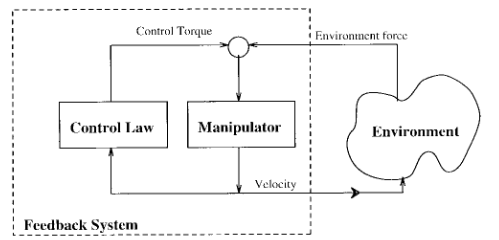
\includegraphics[width=0.48\textwidth]{Images/pvfccontrolloop.png}
    \caption{PVFC loop \cite{li1999passive}}
    \label{fig:pvfccontrolloop}
\end{figure} 
As explained in the paper, a system defined by this supply rate is not passive because obstacles may bring the manipulator to a complete stop for an unbounded amount of time and this loss of kinetic energy cannot be bounded. 
As a result, the passivity relation 
\begin{equation}
    \int_{0}^{t}\tau_{e}^T \dot{q}d\tau \geq -c^2 
\end{equation}
is not valid here because the l.h.s represents the total amount of energy lost to the environment and, as stated before, it cannot be bounded. 
This issue motivates the introduction of an augmented system: a fictitious flywheel is added to the system that acts as an energy storage element.
The dimensionality of the manifold is then increased by one to include the state of the flywheel and this augmented state will be noted as
\begin{align} 
    \bar{q}=[q,q_{\text{fly}}]\\
    \bar{V} = [V, V_{\text{fly}}]
\end{align}

Using such passitive and dissipative systems enables safe interaction between the robot and its environement since the total kinetical energy of the system is bounded by the system initial kinetic energy and energy input from the environement.

\subsubsection{Augmented dynamics}
Let us now describe the dynamics of the augmented system
\begin{equation} 
    \bar{M}(\bar{q})\ddot{\bar{q}} + \bar{C}(\bar{q}, \dot{\bar{q}})\dot{\bar{q}} = \bar{\tau} + \bar{\tau_{e}}
\end{equation}
The mass matrix of the augmented system is defined such that:
\begin{align}
\bar{M}(q) = \begin{bmatrix} 
   M(q) & 0 \\
    0 & m_{\text{fly}}
\end{bmatrix}\\
M(q) =  \begin{bmatrix} 
    m_b & 0 & 0 \\
    0 & m_b & 0 \\
    0 & 0 & m_b \\
 \end{bmatrix}
\end{align}
The Coriolis Matrix of the augmented system is defined such that: 
\begin{align}
\bar{C}(\bar{q}, \dot{\bar{q}}) = \begin{bmatrix} 
    C(q, \dot{q}) & 0 \\
    0 & 0 
\end{bmatrix}
\end{align}
$C$ is built using the Levi–Civita connection described in \cite{li2001passive}.
\subsubsection{Augmented velocity field}
Now let us define the augmented field for the flywheel. The motivation for introducing an augmented system is
to allow energy transfer between the quadcopter actuators and the flywheel such that the total kinetic energy in the system remains constant.
This property is enforced in the definition of the desired velocity field. \\
First let us define $\bar{E}$ to be the total desired energy of the augmented system following the desired velocity field.
$\bar{E}$ can be written as a sum of the flywheel desired kinetic energy $K_{\text{fly}_{d}}$ and the quad desired kinetic energy $K_{quad_{d}}$: 
\begin{equation}
    \bar{E} = K_{\text{fly}_{d}} + K_{quad_{d}}
\end{equation}
Given a desired velocity field $V$ we have: 
\begin{equation}
    K_{quad_{d}}(q) = V(q)^T\frac{1}{2}M(q)V(q)
\end{equation}
Since 
\begin{equation}
    K_{\text{fly}_{d}} = \frac{1}{2} m_{\text{fly}} V^2_{\text{fly}}
\end{equation}
We can derive $V_{\text{fly}}$ in function of  $K_{quad_{d}}(q)$ and $\bar{E}$:
\begin{equation}
    V_{\text{fly}}(q) = \sqrt{\frac{2}{m_{\text{fly}}}(\bar{E}- K_{quad_{d}}(q))} \label{eqn:vfly}
\end{equation}
\subsubsection{PVFC Control law}
To define the PVFC control law, the author defines the following quantities
\begin{align}
    \bar{p}(\bar{q}, \dot{\bar{q}}) = \bar{M}(\bar{q})\dot{\bar{q}} \label{actualaugmomentum}\\
    \bar{P}(\bar{q}) = \bar{M}(\bar{q})\bar{V}(\bar{q}) \label{desiredaugmomentum}\\
    \bar{w}(\bar{q}, \dot{\bar{q}}) = \bar{M}(\bar{q})\dot{\bar{V}} + \bar{C}(\bar{q}, \dot{\bar{q}}) \label{desiredDynamics}
\end{align}
The equation \ref{actualaugmomentum} can be seen as the actual momentum of the augmented system, the equation \ref{desiredaugmomentum} can be seen 
as the desired momentum of the augmented system and \ref{desiredDynamics} is the desired dynamics (desired force applied on) of the augmented system.


From there the author derived the two terms of the coupling control law: 
\begin{align}
    \bar{\tau_c} = \frac{1}{2\bar{E}}(\bar{w}\bar{P}^T - \bar{P}\bar{w}^T ) \dot{\bar{q}} \label{tauc}\\
    \bar{\tau_f} = \gamma(\bar{P}\bar{p}^T - \bar{p}\bar{P}^T ) \dot{\bar{q}} \label{tauf}\\
\end{align}
the $\tau_f$ term is the feedback term, while $\tau_c$ is the term enforcing passivity and allowing to dissipate external forces work into the quadcopter.
The anti-symmetric structure of the matrices multiplying $\dot{\bar{q}}$ is key to proving that the derivative of the kinetic energy in the augmented system is: 
\begin{equation}
    \frac{d}{dt}k(\bar{q}, \dot{\bar{q}}) = \tau_e^T(t)\dot{q}(t) \label{kineticdt}
\end{equation}
This is done by introducing the concepts of compatibility between a metric defining an inner product and an affine connection. It is shown in \cite{li2001passive} that the compatibility between the Levi-Civita connection with the metric defined by $M$ has a direct link between anti-symmetricity of the matrices in the control coupling law, passivity and energy conservation.

From equations \ref{kineticdt} and \ref{passivityCondition}, the passivity of the system with respect to external forces is straightforward.

\subsection{Compensation terms}
When using PVFC with the quadcopter dynamics, it is important to model the effect of drag and gravity on the robot to be able to compensate for them. If those forces are not taken into account, the robot total mechanical energy will decrease until it arrives to a complete stop. 
Therefore, to ensure the robot will continue to follow the desired velocity field, we have to introduce compensation terms for gravity and air drag. 
For simplicity, we chose to model drag as a linear function of the velocity. This worked for our proof of concept but this method 
shows its limits when running the simulation for a greater amount of time because not only drag is not exactly proportional to the speed, but we have no straightforward way of estimating those drag coefficients.
Setting them too high will make our control ouput diverge but setting it too low will make to quad stop following the desired velocity field.  

\section{Implementation}
\label{Implementation section}
As was stated in the introduction, we have two main implementations: 
\subsection{Simplistic Python implementation}
The Python implementation uses simplistic quadcopter dynamics only defined by:
\begin{itemize}
    \item Quad mass: $m_b$
    \item Moments of inertia: $I_{xx}$, $I_{yy}$, $I_{zz}$
    \item drag coefficient: $A_{x}$, $A_{y}$, $A_{z}$
    \item PD attitude gains: $K_{\phi_{p}}$, $K_{\phi_{d}}$, $K_{\psi_{p}}$, $K_{\psi_{d}}$, $K_{\theta_{p}}$, $K_{\theta_{d}}$. $\phi$ is the roll angle, $\theta$ is the pitch angle and $\psi$ is the yaw angle.
\end{itemize}

In this subsection, we will consider $q\in\mathbb{R}_6$ to be the rotational and translational states: $q(t) = (x(t), y(t), z(t), \phi(t), \theta(t), \psi(t))$
and $\dot{q}(t) = \frac{dq}{dt} = (\dot{x}(t), \dot{y}(t), \dot{z}(t), \dot{\phi}(t), \dot{\theta}(t), \dot{\psi}(t))$

It should be noted that the drag coefficients here are used both by the PVFC controller and the dynamics of our system. 
In opposition to the Gazebo implementation, the drag experienced by the quad in the python implementation is also defined by those drag coefficients.
When running in Gazebo, the IRIS model has a real world drag that we do not control.

We use ODEint to evolve the state $(q,\dot{q}, \ddot{q})$ of the system by doing to following on each time step: 
\begin{itemize}
    \item First we compute the current Mass Matrix $M$, Coriolis Matrix $C$, Control Matrix $B$, gravity Matrix $G$. Since the mass of the system is constant, the translational parts of $M$ and $G$ are constants.
    Therefore, the only changes we have to take into account are for $C$ and $B$.
    \item Then we pass to the PVFC controller those dynamics together with the desired velocity field and compute a desired thrust vector.
    \item Given a desired Cartesian thrust vector $\tau_{desired} \in \mathbb{R}_3$, we can decompose it into Euler coordinate $(\alpha, \tau_{\phi_{desired}}, \tau_{\theta_{desired}}, \tau_{\psi_{desired}})$. 
    \item The quad uses a simple attitude PD to compute the final thrust $\tau(t) = (\tau_{{\phi}}(t), \tau_{{\theta}}(t), \tau_{{\psi}}(t)) $ in Euler coordinate :
    \begin{align}
        \tau_{{\phi}}(t) = I_{xx}(K_{\phi_{d}}(\dot{\phi}_{desired} - \dot{\phi}(t))+K_{\phi_{p}}(\phi_{desired} - \phi(t)))\\ \nonumber
        \tau_{{\theta}}(t) = I_{yy}(K_{\theta_{d}}(\dot{\theta}_{desired} - \dot{\theta}(t))+K_{\theta_{p}}(\theta_{desired} - \theta(t)))\\ \nonumber
        \tau_{{\psi}}(t) = I_{zz}(K_{\psi_{d}}(\dot{\psi}_{desired} - \dot{\psi}(t))+K_{\psi_{p}}(\psi_{desired} - \psi(t)))\\ \nonumber
    \end{align}
    \item By multiplying the final Euler thrust by the control matrix, we can obtain the new state of the quadcopter
\end{itemize}
It is important to notice that the big difference between the python implementation and the ROS/Gazebo/PX4 that we will later detail is that we do not explicitly use a PD attitude gains in the latter. 
The PX4 firmware of the IRIS model has its own low level attitude controller.


The desired velocity fields are computed using Sympy (A Python library for symbolic calculations) for easy field and field gradient computation. Since most fields we used are derived from potential functions, we can easily obtain the field and field Jacobian required by PVFC by symbolically differentiating their potentials or shaping functions.

\subsection{Full Sensor Placement pipeline in ROS/Gazebo/Pixhawk 4}
In this implementation, we are using a real world quadrotor called IRIS quad provided in the Pixhawk 4 SITL package. 
The dynamics are evolved and computed by Gazebo. 
The implementation is divided in 2 ROS Nodes, 1 ROS-PCL Node, 1 Gazebo-ROS plugin, and 1 Pixhawk 4/MAVROS node.
A diagram of the implementation is shown in figure \ref{fig:implementationdiagram}.
\subsubsection{Velocity Field ROS Node}
This node subscribes to the MAVROS odometry topic, computes the velocity field at the current position and publishes the desired field and field gradient. 
We implemented all the velocity field using the symbolic math library SymEngine so that all gradient computations from potential or shaping function would be done automatically. 
In addition, this node is implementing a state machine such that in each state, a specific field is being used.
Specifically, the first state gives a sink to get altitude, the second state is a sink field to approach the target, 
the third state represents the contact phase with the wall (the node subscribes to a topic called ``grasping`` to know if the grasping arm is currently activated). It starts when an engagement signal is received from the grasping arm, and it finishes when a disengagement signal is received from the grasping arm. 
The last state is to get away from the wall and land, we use a sink field to implement it.
We implemented an obstacle avoidance system for generic superquadratic obstacles, upon obstacle detection, we compute the avoidance field for this obstacle from the appropriate shaping function, an irrotational field is generated to avoid the obstacle. This node subscribes to an obstacle topic to know when new obstacles have been detected. 
\subsubsection{PVFC ROS Node}
This node subscribes to the desired velocity field and to the MAVROS odometry and publishes a thrust vector on the MAVROS attitude topic computed by the PVFC controller. The output of the passive velocity field controller is a 4-dimensional vector containing the desired thrust to be applied in each direction $(x,y,z, fly)$ including the thrust to be applied on the fictitious flywheel. 
However, the input control for the IRIS model needs a desired attitude and thrust amplitude. Therefore, after obtaining the desired (Cartesian) thrust vector from PVFC, we convert it to desired Euler angles with desired amplitude $(\alpha, roll, pitch, yaw)$. 
We can then convert this pose to quaternion and publish it to the attitude topic of the IRIS quad.
It should be noted that the thrust amplitude expected by the IRIS attitude control is not in Newtons but is a scalar between 0 and 1. As a result, we had to experimentally calibrate a thrust slope and thrust intercept (affine transformation) to map the desired PVFC thrust amplitude to a scaled thrust amplitude. 
\subsubsection{PCL Object Segmentation Node}
This node reuses the code of a PCL \href{https://pcl.readthedocs.io/projects/tutorials/en/master/cylinder_segmentation.html}{tutorial} performing cylinder segmentation on point cloud data. 
We added a ROS integration to the velocity field topic the position of the detected object and also we implemented the transforms from camera point of view to FCU (Flying control unit) frame, and from FCU frame to world frame. 
It works in the following way:
\begin{itemize}
    \item Use a PCL passthrough filter to remove Nan datapoints and the scene background
    \item Use the PCL NormalEstimation class to estimate the normals of the cleaned point cloud scene. This is done using KdTree based methods for increased robustness against noise in the measurements. KdTrees are data structures used in Computer Science that are very efficient for nearest neighbor search
    \item Perform plane model segmentation on the extracted normals using RANSAC and filter out the planar inliers
    \item After the last step, we should have clean normals containing only cylinders normals, we can now use the SACSegmentationFromNormals class of PCL to extract the coefficient of the cylinder and its position in the frame of the camera
    \item If a cylinder was detected, we transform the position of the cylinder from the depth camera frame to the gazebo world frame, and we publish it to the cylinder topic for the velocity field node to update the desired velocity field
\end{itemize}
\subsubsection{Grasping arm Gazebo-ROS plugin}    
This node reuses the code of the vacuum arm of Gazebo, but it was modified so that could be attached to the moving IRIS model and fixed to a wall in Gazebo. 

\begin{figure*}[h!]
    \centering
    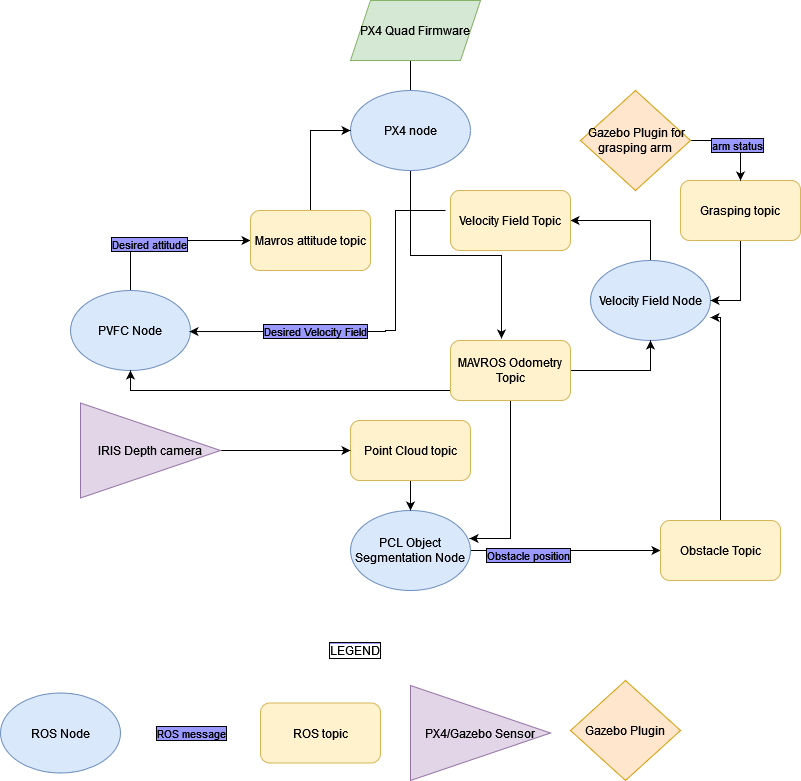
\includegraphics[width=\linewidth]{Images/implementation diagram.png}
    \caption{implementation diagram}
    \label{fig:implementationdiagram}
\end{figure*}
\newpage

\section{Results, Evaluation and Experiments}
\subsection{$\ast$ abstract}
\subsection{Introduction}
 \begin{itemize}
    \item general motivation/background of this study: 
    \item PVFC controller (l)
    \item Implementing this controller requires velocity field , that is updated based on current position.
          someone studied velocity field using potential, briefly describes the main principle. 
           Explain why this technique is suitable/beneficial to your project (compared to other methods for velocity field).
    \item Calibrate thrust
    \item  error within the framework of this controller due to the neglecting gravity and friction
          someone did a study on compensating for these errors, briefly introduce the principle. The right amout of (Ax Ay Az) 
          can improve ... performance. However, ... diverge ... also talk about  beta 
    \item PCL: 
    \item Gazebo modified : arm, pcl modified
 \end{itemize}

%  \subsection*{future work}
%   \begin{itemize}
%     \item estimate optimal parameters of E_bar, Gamma gains, a's to reduce input-output difference
%   \end{itemize}
\section{Conclusion, Future Work}
In this project, we presented an application of a passive velocity field controller to the sensor placement task with a grasping arm mounted on a quadcopter integrated with a depth camera for active obstacle avoidance. 
We first implemented a simple passive velocity controller with simple dynamics on Python using Sympy to symbolically derive and evaluate the dynamics and velocity fields. 
This implementation allowed us to reproduce results from the PVFC paper \cite{li1999passive}.
Then we implemented the full pipeline of sensor placement using ROS, PX4, Gazebo and PCL and explained the different field\\

Because of lack of time, we could not improve the implementation but many steps could have been done to make it more robust.
First, the linear approximation for the drag coefficient we used seems to be task specific and may need to be updated during flight. Therefore, another controller could be used to tune the linear drag coefficient 
according to the total mechanical energy in the augmented system.\\
In addition, we often struggled to choose a value for the gains parameter of PVFC $\bar{E}$ and $\gamma$. Multiple strategies could be used to solve this problem such as sampling the velocity field to know the minimum $\bar{E}$ required 
such that the flywheel velocity never becomes an imaginary number. \\
It would be also possible to think about an evolutionary algorithm based solution for finding the best gains for the task. For example, in the case of a contour following task, a fitness function could be defined as a function of the path tracking accuracy.
Another improvement could be to generalize the superquadratic detection spectrum to be able to detect any kind of superquadratic.\\
It would also be possible to switch to a solenoidal field in case the quad is stuck at the local minimum in the velocity field.\\
The yaw angle of the quad for all experiments but the depth camera has a limited field of view, to always be able to detect obstacle in the direction of movement, it would be necessary to set the desired yaw angle to be in the direction of the desired velocity field.
Finally, in a real world situation we may not have access to a grasping arm to place a sensor therefore we would need to use the spherical velocity field developed in section 3. We implemented this field with SymEngine but did not have time to integrate in with our Gazebo experiment. 

The ethics checklist has been checked and all items have been ticked ``No`` except for the potential military application.
We did not use any human, embryos, personal data, animals. The project was entirely developed in the UK, no environmental safety issues.
We only used open sourced software.
However, this project could have potential military applications but I sincerely hope for the military that they have better options.

\section{Running the code}
The PVFC python implementation is available in \href{https://github.com/bsbretly/pvfc_sim/tree/devel-beta_error}{this branch}.\\
The PVFC ROS implementation is available in \href{https://github.com/bsbretly/pvfc_ws/tree/jonas-pcl}{this branch}.
For both of them, a readme is available describing how to run it. 
In addition, a playlist of videos detailing how to run the experiments on the ROS/Python implementation is provided \href{https://www.youtube.com/watch?v=tSBsaKx5Zww&list=PLvZGCthLI9WrbS7W-F28ljQfRyHxxw-9p}{here}.

\newpage
%\clearpage                                     % Sometimes you want the rest on separate pages.

%%%%%%%%%%%%%%%%%%%%%%%%%%%%%%%%%%%%%%%%

% Bibliography
%--------------------
\printbibliography

\end{document}

% Copyright Remarks:
%--------------------

% Copyright holder: Vebjørn S. Førde, copyright: CC BY 4.0
% Note: The author of this template is also the copyright holder.

% Below is an explanation of the CC BY 4.0. Additional statements/ 
% clarifications made by the author/copyright holder are marked with *.

% YOU ARE FREE TO:
% Share — copy and redistribute the material in any medium or format
% Adapt — remix, transform, and build upon the material
% for any purpose, even commercially.

% UNDER THE FOLLOWING TERMS:
% Attribution* — You must give appropriate credit, provide a link to the license,
% and indicate if changes were made. You may do so in any reasonable manner, but 
% not in any way that suggests the licensor endorses you or your use.

% *Note: I do not need credit when the template is used to make a PDF document
% that is then distributed (like handing in a lab report). However, I would
% like for you to give credit if you choose to distribute the "software" 
% (the associated documentation files, .tex files and such). If you distribute
% both the PDF and the software, then you only need to give credit in the software
% distribution.
% I do not need credit for the plain text (text in output PDF). However, you should
% give me credit if you chose to use/ distribute any of the images in this document.

% No additional restrictions — You may not apply legal terms or technological 
% measures that legally restrict others from doing anything the license permits.

% NOTICES:
% No warranties are given.

% Disclaimer* (added by copyright holder):
% THE SOFTWARE IS PROVIDED "AS IS", WITHOUT WARRANTY OF ANY KIND, EXPRESS OR
% IMPLIED, INCLUDING BUT NOT LIMITED TO THE WARRANTIES OF MERCHANTABILITY,
% FITNESS FOR A PARTICULAR PURPOSE AND NONINFRINGEMENT. IN NO EVENT SHALL THE
% AUTHORS OR COPYRIGHT HOLDERS BE LIABLE FOR ANY CLAIM, DAMAGES OR OTHER
% LIABILITY, WHETHER IN AN ACTION OF CONTRACT, TORT OR OTHERWISE, ARISING FROM,
% OUT OF OR IN CONNECTION WITH THE SOFTWARE OR THE USE OR OTHER DEALINGS IN THE
% SOFTWARE.

% Read more about CC BY 4.0:
% https://creativecommons.org/licenses/by/4.0/